\chapter{Digital Video Interface}
\gls{dvi} is a video interface which surfaced in 1999. Designed by the \gls{ddwg} as a replacement for \gls{vga}, it was mainly used to display output from a computer's graphics adapter onto a monitor, although it did see some limited use in other entertainment equipment such as TVs and DVD players. Despite its age, the interface has more than enough bandwidth for 1080p RAW video and its relative simplicity makes it an attractive base for transferring image sensor data.

\section{Interface overview}

\begin{figure}
  \centering
  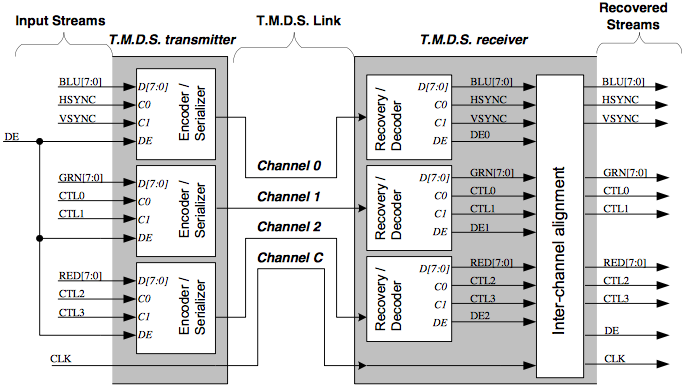
\includegraphics[width=1\textwidth]{./img/dvi_link_overview.png}\par
Source: DVI 1.0 Specification
  \caption{Dual-link \gls{dvi} system}
  \label{fig:dvi_link_overview}
\end{figure}

\subsection{Video format and timing}
\marginpar{Hsync + Vsync + blanking, 8-bits per-pixel}
\subsection{Physical layer}
\subsection{DDC and EDID}

\section{Required additions for image sensors}